% Created 2020-09-16 Mi 20:28
% Intended LaTeX compiler: pdflatex
\documentclass[a4paper,11pt]{article}
\usepackage[latin1]{inputenc}
\usepackage[T1]{fontenc}
\usepackage{graphicx}
\usepackage{grffile}
\usepackage{longtable}
\usepackage{wrapfig}
\usepackage{rotating}
\usepackage[normalem]{ulem}
\usepackage{amsmath}
\usepackage{textcomp}
\usepackage{amssymb}
\usepackage{capt-of}
\usepackage{hyperref}
\usepackage{pgfplots}
\author{Moaz Haque, Felix Oechelhaeuser, Leo Pirker, Dennis Schulze}
\date{\today}
\title{Analysis I und Lineare Algebra f�r Ingenieurwissenschaften \large  \\ Hausaufgabe 07 - Geuter 29}
\hypersetup{
 pdfauthor={Moaz Haque, Felix Oechelhaeuser, Leo Pirker, Dennis Schulze},
 pdftitle={Analysis I und Lineare Algebra f�r Ingenieurwissenschaften \large  \\ Hausaufgabe 07 - Geuter 29},
 pdfkeywords={},
 pdfsubject={},
 pdfcreator={Emacs 27.1 (Org mode 9.3.6)}, 
 pdflang={English}}
\begin{document}

\maketitle
\tableofcontents

\pagebreak

\section{Aufgabe 1}
\label{sec:org51b6dca}
\subsection{a)}
\label{sec:org0f46703}
Es gilt

\begin{align*}
  \frac{1}{b} + \frac{1}{g} &= \frac{1}{f} \\
  \Leftrightarrow \frac{1}{b} &= \frac{g - f}{fg} \\
  \Leftrightarrow b &= \frac{fg}{g - f}
\end{align*}

Damit ist b betrachtet als Funktion

$$ b(g) = \frac{fg}{g - f} $$

\subsection{b)}
\label{sec:org9ef8c25}
Da der Bruch nur f�r alle \(g \neq f\) definiert ist, \\
ist b nur auf \(\mathbb{R}\) $\backslash$ \{\(f\)\} stetig.

\subsection{c)}
\label{sec:org0558c2b}
Es gilt f�r den ersten Term

\begin{align*}
  \lim_{g \rightarrow \infty} b(g) &= \lim_{g \rightarrow \infty} \frac{fg}{g - f} \\
  &= \lim_{g \rightarrow \infty} \frac{f}{1 - \frac{f}{g}} \\
  &= \frac{f}{1 - 0} \\
  &= f
\end{align*}

Es gilt f�r den zweiten Term

\begin{align*}
  \lim_{g \rightarrow f} b(g) &= \lim_{g \rightarrow f} \frac{fg}{g - f} \\
  &= \frac{\lim_{g \rightarrow f} fg}{\lim_{g \rightarrow f} (g - f)} \\
  &= \frac{f^2}{f - f} \\
  &\Rightarrow \lim_{g \rightarrow f} b(g) = \infty
\end{align*}

\section{Aufgabe 2}
\label{sec:org0b84461}
\subsection{a)}
\label{sec:org27a602b}
Es gilt f�r \(\lim_{x \rightarrow 1^-} f(x)\)

\begin{align*}
  \lim_{x \rightarrow 1^-} f(x) &= \lim_{x \rightarrow 1^-} (\cos(\pi x) + 3) \\
  &= \cos(\pi) + 3 = -1 + 3 = 2
\end{align*}

und es gilt f�r \(\lim_{x \rightarrow 1^+} f(x)\)

\begin{align*}
  \lim_{x \rightarrow 1^+} f(x) &= \lim_{x \rightarrow 1^+} \frac{x^2 + 1}{x + 1} \\
  &= \frac{1^2 + 1}{1 + 1} = \frac{2}{2} = 1
\end{align*}

daraus folgt, dass \(f\) an der Stelle \(x = 1\) nicht stetig ist. \\

\ldots{} \\

Damit ist \(f\) auf \(\mathbb{R}\) $\backslash$ \{1\} stetig.

\subsection{b)}
\label{sec:org0a41091}
\begin{itemize}
\item Punkte an Intevallgrenzen (P\textsubscript{1}(-1, -1) und P\textsubscript{2}(2, ln(2)))
\item einsetzten in \(s(x) = y_1 + \frac{y_2 - y_1}{x_2 - x_1}x\)
\end{itemize}

\section{Aufgabe 3}
\label{sec:org3eda6d7}
\subsection{a)}
\label{sec:org8f18cc1}
\begin{itemize}
\item Intevallgrenzen einsetzten in f
\item f ist stetig und differenzierbar
\item Folgerung: Nullstelle
\end{itemize}

\subsection{b)}
\label{sec:orge39c759}
\section{Aufgabe 4}
\label{sec:org49de035}
\subsection{a)}
\label{sec:org28a828c}
\subsection{b)}
\label{sec:org5e04caa}
\subsubsection{a}
\label{sec:org0529144}
$$ (5x^3 - 2\sin(3x))' = 15x^2 - 6\cos(3x) $$

\subsubsection{b}
\label{sec:org42b239c}
$$ (\cos(x) e^x)' = \cos(x)e^x - \sin(x)e^x $$

\subsubsection{c}
\label{sec:org1fc60c4}
$$ (e^{2x^2+11} + 7)' = 4x e^{2x^2+11} $$

\subsubsection{d}
\label{sec:orga81bad5}
$$ \left( \frac{\sin(x^2 - 2\pi)}{\cos(3\pi - x^2)} \right)' = \frac{-2x}{\cos^2(3\pi - x^2)} $$

\section{Aufgabe 5}
\label{sec:orgcc775e9}
F�r die 1. Ableitung von \(f\) gilt

$$ f'(x) = -\frac{2}{(x-2)^2} $$

dann gilt f�r eine beliebige Tangente \(t(x) = ax + b\) am Graphen von \(f\)

\begin{align*}
  a &= f'(x_0) = -\frac{2}{(x_0-2)^2} \\
  b &= f(x_0) - f'(x_0) \cdot x_0 = \frac{2}{x_0-2} + 2 + \frac{2 x_0}{(x_0-2)^2}
\end{align*}

mit der Anforderung, dass \(a = -\frac{1}{2}\) sein muss. Damit gilt

\begin{align*}
  a = -\frac{2}{(x_0-2)^2} &= -\frac{1}{2} \\
  \Leftrightarrow \frac{(x_0-2)^2}{2} &= 2 \\
  \Leftrightarrow (x_0-2)^2 &= 4 \\
  \Leftarrow x_0 - 2 &= \pm 2
\end{align*}

daraus ergeben sich die beiden Stellen \(x_1 = 0\) und \(x_2 = 4\). Daraus folgen dann die beiden Tangenten

\begin{align*}
  t_1(x) &= -\frac{1}{2}x + 1 \\
  t_2(x) &= -\frac{1}{2}x + 5
\end{align*}

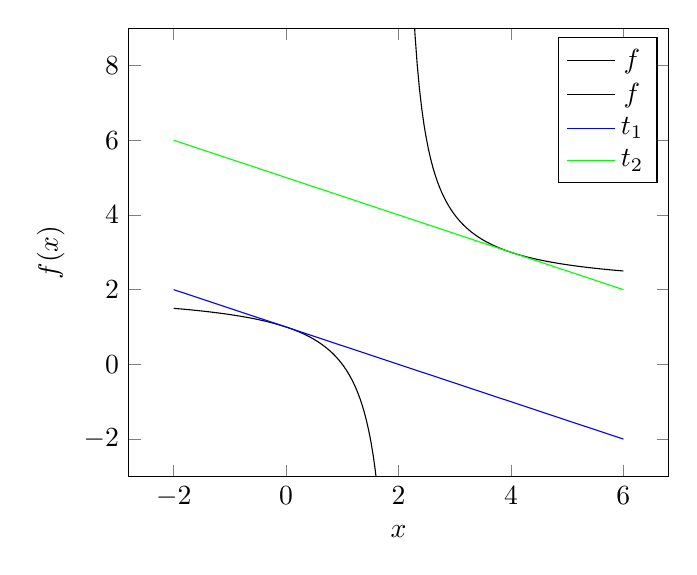
\begin{tikzpicture}
  \begin{axis}[xlabel = $x$, ylabel = {$f(x)$}, ymin=-3, ymax=9]
  \addplot[samples=100, color=black, domain=-2:1.99]{2/(x-2) + 2};
  \addplot[samples=100, color=black, domain=2.01:6]{2/(x-2) + 2};
  \addlegendentry{$f$}
  \addlegendentry{$f$}
  \addplot[color=blue, domain=-2:6]{-1/2 * x + 1};
  \addlegendentry{$t_1$}
  \addplot[color=green, domain=-2:6]{-1/2 * x + 5};
  \addlegendentry{$t_2$}
  \end{axis}
\end{tikzpicture}

\section{Aufgabe 6}
\label{sec:org6bce14b}
\subsection{a)}
\label{sec:org0427af6}
\subsection{b)}
\label{sec:org7e9bb79}
\end{document}